
This chapter now turns to the physical principles that enable satellites to
sense clouds and precipitation from space. The remote sensing of any atmospheric
quantity is based on its interaction with electromagnetic radiation. The
measured radiation can be used to infer physical properties of atmospheric
quantities by inverting the interaction between radiation and the atmosphere.
Doing so, requires a quantitative model of the propagation of radiation through
the atmosphere. Such a model is provided by the physical theory of radiative
transfer.

Since radiative transfer theory is fundamental to atmospheric remote sensing ,
this section provides an introduction to radiative transfer in the atmosphere.
The focus is put on the interaction of radiation with hydrometeors. This
presentation is mostly based on the more comprehensive texts by Mishchenko et
al. (2002), Thomas and Stamnes (2002), and Wallace and Hobbs (2006).


\section{Radiative transfer theory}

Radiative transfer theory describes the propagation of electromagnetic radiation
through a medium. It provides simplified model of the electromagnetic and
quantum mechanical interactions of a perfectly monochromatic beam of light.
Electromagnetic sensors measure the mean total energy that is transferred by
electromagnetic radiation as well the correlations between the components of the
beam's electric field, which define the beam's \textit{polarization state}. The
radiation measured by a sensor at position $\bm{r}$ pointing in direction
$\bm{-n}$ is fully described by the four dimensional stokes vector
\begin{align}
  \bm{I}(\bm{r}, \bm{n}) &= \left [ \begin{array}{c}
    I \\
    Q \\
    U \\
    V \\
    \end{array} \right ]
\end{align}

The components $I, Q, U$ and $V$ are called the stokes parameters and have the
unit of monochromatic energy flux. The stokes vector fully describes the state
of a monochromatic beam of radiation to the extent that it can be measured by an
electromagnetic sensor. Thus any electromagnetic measurement observation from
knowledge of the stokes vector at the position of the sensor. Radiative transfer
theory describes how the stokes vector changes as it propagates through a medium.

\subsection{Interactions with matter}

Radiative transfer theory distinguishes three fundamental processes through
which matter interacts which radiation. These are (1) the emission of
electromagnetic radiation, (2) its absorption and (3) scattering.

\subsubsection{Emission}

At temperatures above absolute zero, all matter emits radiation through the
process of thermal emission. Thermal emission occurs when matter transitions
from a quantum mechanical state of higher energy to one of lower energy which
causes the excess energy to be emitted in the form of radiation. The amount of
radiation of a given frequency $\nu$ emitted by a body depends on its
temperature and material. It is typically modeled using a material-dependent
emissivity vector $\vec{e}$, which relates the emission of the material to that
of an ideal black body, i. e. a material that absorbs all incoming radiation:
 \begin{align}
   \label{eq:emissivity}
   \vec{I} &= (\vec{e} \cdot ds) B(T, \nu)
 \end{align}
 Here $B(T, \nu)$ is the radiation emitted by a black body at temperature $T$
 and frequency $\nu$, which is described by Planck's law
 \begin{align}
   B(T, \nu) &= \frac{2 \nu^2}{c^2}\frac{h\nu}{e^{\frac{h\nu}{k T}} - 1},
 \end{align}
 with $c$ is the speed of light in vacuum, $h$  the Planck constant and $k$
 the Boltzmann constant.

The emissivity vector defined above is a differential quantity that describes
emission from a volume element along an infinitesimal step along the propagation
path. This means that in order to obtain the emission from a finite volume, the
emission must be integrated along the propagation path. For a material that is
opaque, there is no need to integrate over the full volume, since only its
surface will contribute to the observed emission. The emissivity of a surface
can be described using an emissivity vector $\vec{e}$ in the same way as for
emission from a volume, with the difference that its components are unitless
and integration over the propagation path is not required.

\subsubsection{Absorption}

Absorption refers to the process of radiation being converted into internal
energy of the matter it interacts with. Mathematically, this process is
described by the absorption vector $\vec{\alpha}$, defined as the fraction of
the incoming radiation that is absorbed along an infinitesimal distance $ds$
along the propagation path:
\begin{align}
\vec{I}_\text{absorbed} &= (\vec{\alpha} \cdot\ ds) \odot \vec{I}
\end{align}
Here $\odot$ denotes the element-wise product of the absorption vector and
the Stokes vector $\vec{I}$ of the incoming radiation. Absorption may be
understood as the inverse process of thermal emission. Formally, this is
expressed by Kirhoff's  law of radiation
\begin{align}
  \vec{\alpha} &= \vec{\epsilon},
\end{align}
which states that the absorption vector is identical to the emissivity vector
defined in Eq.~\ref{eq:emissivity}. This law is applicable to all matter in the
atmosphere given that it is in a state of local thermal equilibrium (LTE). LTE
occurs when the density of matter is sufficiently high so that the population
rates of energy states above the ground state are determined by thermal
collisions rather than the absorption of radiation. This decouples the emission
of radiation from the radiation field itself, allowing the simplified treatment
of matter as thermal emitters with the emission rates independent of the
radiation field. LTE is a valid assumption for radiative transfer in the
troposphere.

\subsubsection{Scattering}

Scattering describes the effect of inhomogeneities in the dielectric properties
of the medium on the propagation of the beam. When a plane-parallel
electromagnetic wave encounters such inhomogeneities, it is scattered in all
directions. Since parts of the energy flux of the beam are deviated from the,
the intensity of the radiation along the beam is decreased. As it propagates
through the medium, the intensity of a beam is thus decreased by the effects of
absorption and scattering. The combination of these two processes is referred to
as attenuation or extinction. In the presence of other light sources, scattering
of radiation into the beam in acts to increase its intensity.

Mathematically, the scattering of a beam of light propagating in direction
$\vec{n}$ into the direction $\vec{\hat{n}}$ is described by the phase
matrix $\mat{Z}(\vec{\hat{n}}, \vec{n})$:
\begin{align}
  \vec{I}_\text{scattered}(\vec{\hat{n}}) &= \mat{Z}(\vec{\hat{n}}, \vec{n}) \vec{I}(\vec{n})
\end{align}
The combined, attenuating effects of scattering and absorption are given by
the attenuation matrix $\mat{K}$, which is the sum of the absorption vector
$\vec{\alpha}$ and the fraction of radiation scattered away from the propagation
path:
\newcommand*{\vertbar}{\rule[-1ex]{0.5pt}{2.5ex}}
\newcommand*{\horzbar}{\rule[.5ex]{2.5ex}{0.5pt}}
\begin{align}
  \vec{K} &=
  \left [ \begin{array}{cccc}
      \vertbar & \vertbar & \vertbar & \vertbar \\
      \vec{\alpha} & \vec{0} & \vec{0} & \vec{0} \\
      \vertbar & \vertbar & \vertbar & \vertbar
    \end{array} \right ]
       + \int_{\vec{\hat{n}}} d\vec{\hat{n}}\ \mat{Z}(\vec{\hat{n}}, \vec{n})
\end{align}


\subsection{The radiative transfer equation}

The previous section introduced the fundamental interactions of radiation
with matter and how they are described mathematically in radiative transfer
theory. Combining the three processes of emission, absorption and scattering,
the change that a beam undergoes as it travels a distance $ds$ along its
propagation path through the atmosphere is described the vector radiative
transfer equation (VRTE):
\begin{align}\label{eq:vrte}
  \frac{d\vec{I}(\vec{n})}{ds} &=
  -\mat{K}\vec{I}(\vec{n}) + \vec{\alpha} \cdot B_\nu(T) + \int_{\hat{\vec{n}}} d\hat{\vec{n}} \ \mathbf{Z}(\vec{n}, \vec{\hat{n}}) \vec{I}(\vec{\hat{n}}).
  \end{align}

The first term on the right hand side is the extinction term, which represents
the combined effects of absorption and scattering of radiation out of the
propagation direction, and thus acts to decrease the intensity of the radiation
along the line of sight. The second term represents emission along the line of
propagation, with the emissivity vector $\bm{\epsilon}$ replaced by the
absorption vector $\bm{a}$ according to Kirchoff's law of thermal radiation. The
third term represents the radiation that is scattered into the line of sight.
Both of these terms act to increase the intensity along the line of sight.

\section{Observations of hydrometeors}

The remote sensing of hydrometeors\footnote{%
Hydrometeor is the collective term for the liquid and frozen particles that
 that make up clouds and precipitation.
}
is based on their interaction with radiation.The relation of the physical
properties of hydrometeors to the processes of absorption and scattering define
the extent to which observations can inform us about them. Since these
relationships depend on the wavelength $\lambda$ of the radiation, observations
across the electromagnetic spectrum are sensitive to different types and
properties of hydrometeors.
%
\begin{figure}[!hbpt]
  \centering
  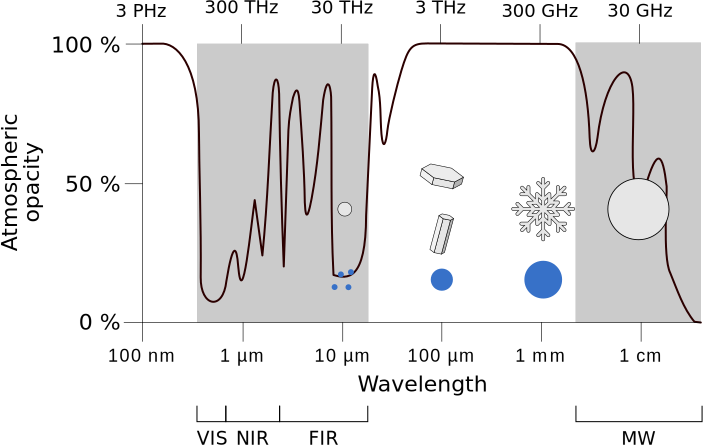
\includegraphics[width=0.75\textwidth]{spectrum}
  \caption{Overview of the electromagnetic spectrum used for hydrometeor retrievals. The black
    curve shows the variation of the atmospheric opacity across the spectrum.}
  \label{fig:radiative_transfer:spectrum}
\end{figure}
%
The discussion presented here focuses on observations from the visible (VIS,
$\SI{350}{\nano \meter} \leq \lambda < \SI{720}{\nano \meter}$), infrared (IR,
$\SI{0.72}{\micor \meter} \leq \lambda < \SI{20}{\micro \meter}$), and microwave
(MW, \SI{1}{\milli \meter} \leq \lambda < \SI{1}{\meter}$) regions, which are
most commonly used for the remote sensing of clouds and precipitation.

An overview of the electromagnetic spectrum is provided in
Fig.~\ref{fig:radiative_transfer:spectrum}. The graph provides an approximate
description of the atmospheric opacity across different wavelengths of the
electromagnetic spectrum. When viewed from a satellite, the atmospheric
opacity defines how far down into the atmosphere a sensor can 'see'. Generally,
where the opacity is low, the satellite can see down to the surface, while where
it is high it is sensitive only to the upper parts of the atmosphere.

\subsection{The atmospheric background}

Satellite observations are sensitive not only to clouds but also to the
gases and aerosols in the atmosphere. As a first approximation the
observations in the absence of clouds, so called \texit{clearsky} scenes,
may be viewed as the background upon which clouds are observed.

Observations at short wavelengths differ from those at long wavelengths with
respect the source of the observed radiation. At wavelengths in the visible and
near infrared regions, the largest part of the observed radiation stems from the
sun. This is because, at these short wavelengths, black body radiation at
typical atmospheric temperatures is small compared to reflection of solar
radiation. As the wavelength increases, the intensity of solar radiation decreases
while that of a black bodies at atmospheric temperatures increases. At wavelengths
exceeding $\approx \SI{3}{\micro \meter}$ emission from atmospheric constituents
dominates the intensity of reflected solar radiation. This threshold separates
the thermal ($\lambda \geq \SI{3}{\mico \meter}$) from the near infrared. At
these wavelengths solar emission can generally be neglected and all observed
radiation originates from the atmosphere itself or the Earth's surface.

The atmospheric opacity displayed in Fig.~\ref{fig:radiative_transfer:spectrum}
corresponds to the combined effects of absorption and extinction by gases in the
atmosphere. Gases affect radiation mostly through absorption and emission, while
scattering plays a role only in the visible range. The reason for this is the
small size of the molecules (around $\SI{1}{\nano \meter}$) compared to the
wavelengths of the radiation.

There is little absorption in the visible range with most of it due to water
vapor. In the near and thermal infrared absorption increases but is concentrated
in discrete absorption bands, which makes the opacity of atmosphere highly
variable across wavelengths. The principal gaseous absorbers in the infrared
region are water vapor, cabon dioxide and ozone. Absorption also plays an
important role in the microwave region with significant contributions from water
vapor, oxygen and ozone. 

In addition to the effects of gases, satellite observations can be affected by
the presence of aerosols. Aerosols are significantly larger than the gas
molecules in the atmosphere and therefore affect both VIS and IR observations
through scattering. In the shortwave part of the electromagnetic spectrum, which
is dominated by solar radiation, aerosols reflect incoming solar radiation and
which typically increases the intensity of the measured radiation due to the
relative darkness of the surface. In the longwave infrared region, the
scattering of aerosols acts to decrease the intensity of the upwelling radiation
from the surface and the lower parts of the atmosphere. Aerosols have no
significant effect on microwave observations.

\subsection{Physical properties of hydrometeors}

Also displayed in Fig.~\ref{fig:radiative_transfer:spectrum} are the principal
classes of hydrometeors located at the wavelengths corresponding to their
approximate sizes. Liquid hydrometeors are identified using blue coloring, while
white corresponds to frozen hydrometeors.

Among the smallest hydrometeors are liquid cloud droplets with typical sizes
around $\SI{10}{\micro \meter}$. These droplets make up liquid clouds. At sizes
of around $\SI{100}{\micro \meter}$ water drops become large enough to fall out
of the clouds. The smallest precipitating liquid droplets are drizzle. These
drops have characteristic sizes of around $\SI{100}{\micro \meter}$. Rain drops
are larger with typical drop sizes around $\SI{1}{\milli \meter}$.

Very small frozen hydrometeors typically form though homogeneous freezing at
temperatures below $-\SI{36}{\degree \celsius}$. Since they require very low
temperatures to form, these hydrometeors are only found at high altitudes.
Larger ice crystals typically form at higher temperatures and lower altitudes.
These range in size from $\SI{100}{\micro \meter}$ to $\SI{1}{\milli \meter}$.
Snow flakes are aggregates of ice crystals that form through collision. These
rang in size from several millimeters to centimeters. When snowflakes fall through
layers that are supersaturated with respect to liquid water, the water vapor
condenses upon the snowflakes causing further growth through a process called
riming. Rimed snowflakes are referred to as graupel and have typical sizes
of $\SI{1}{\centi \meter}$.  Finally, the largest hydrometeors are hailstones,
which form only in strong thunderstorms and can reach sizes of up to
$\SI{10}{\centi \meter}$$.


%Most observations of clouds are affected not only by the clouds themselves but
%also by other constituents of the atmosphere. In the following, we will
%therefore first discuss observations without clouds, so called \textit{clear
%  sky} observations, as these form the background for the observations of
%hydrometeors. This is followed by a discussion of the observable effects of
%hydrometeors on the observations, which gives rise to the signal in the
%\textit{all-sky observations} that can be used to infer the physical properties
%of hydrometeors.

%\subsection{The Earth's surface}
%
%The characteristics of the Earth's surface vary considerably across the
%electromagnetic spectrum. In the visible range, the surface absorbs large parts
%of the radation. The darkest surfaces are the ocean which absorbs around
%$\SI{95}{\percent}$ of the incoming radiation. Bare land surface and forests are
%considerable brighter but still absorb most ($\approx \SI{75}{\percent}$) of the
%incoming radiation. In contrast to that, snow and ice covered surface reflect
%nearly all of the incoming radiation and thus appear very bright.
%
%In the infrared region of the electromagnetic spectrum the emissivity of the Earth surface
%increases significantly. For wavelengths between $3$ and $\SI{20}{\micro \meter}$ the emissivity
%of most surface types is larger than $0.9$. At these wavelengths the surface is very effective at
%emitting and absorbing radiation and there is little contrast between different surface types.
%
%In the microwave region surface emissivity patterns are more complex. Emissivity
%from land is relatively high, while emissivity from water surfaces is low. The
%contrast between land and surface increases with the wavelength. Emissivities
%from snow and ice are lower than that of most bare land surface but higher than
%that of water. The emissivity furthermore depends on the viewing angle and the
%polarization of the radiation.
%
%While these general tendencies are helpful for a qualitative analysis of
%satellite imagery, it should be noted that they only provide a rough
%characterization of the behavior of the Earth's surface across the
%electromagnetic spectrum. Accurate, quantitative modeling of surface
%emissivities is still an unsolved problem and thus remains an area of
%active research.

\subsection{Cloudy sky}

Due to their comparably large sizes, the scattering effects of hydrometeors need
to be taken into account across most wavelengths from the VIS to the MW regions.
In the VIS and NIR there is little absorption from either water or ice.
Hydrometeors thus mostly deviate radiation from its propagation path without
significantly decreasing its intensity. Clouds observed at these wavelengths
appear bright because the solar radiation scattered back towards the sensor is
much more intense than what is reflected from the surface.

In the FIR region, both water and ice are strongly absorbing. Because the
ambient temperature decreases with altitude in the troposphere, opaque clouds
emit less intense radiation than the surface or water vapor below them.
At wavelength at which there is weak absorption from water vapor, so called
\textit{window channels}, radiation from opaque clouds can be used to
infer the temperature at the cloud top, which is related to the altitude of
the cloud.

At microwave frequencies, liquid water is a much more efficient absorber than
ice. Because of this, absorption and emission from ice can be neglected. At
frequencies below $\sim \SI{50}{\giga \hertz}$, the scattering from hydrometeors
becomes negligible. Because of that the dominant impact of hydrometeors on
satellite observations is through the emission from liquid hydrometeors. Over
Ocean surfaces, which have low emissivity and thus emit little radiation, the
emission from liquid hydrometeors causes a clear signal in microwave
observations at these low frequencies.

At frequencies above $\SI{50}{\giga \hertz}$, observations become
sensitive to the scattering from snow flakes. This scattering signal is
important for sensing precipitation over land, where the emission signature from
liquid hydrometeors may not be detectable due to the much warmer background
surface.

\section{Satellite remote sensing}

Just as the interaction of hydrometeors with electromagnetic radiation,
also the information content of the satellite observations  on specific
hydrometeors varies with the wavelength. However, the observation frequency
can in general not be chosen freely but is subject to technological
limitations, which affect characteristics such as spatial and temporal
resolution of the observations.


\subsection{Satellite orbits}

The satellite orbit in which the satellite and sensor are placed plays an
important role in determining the characteristics of the resulting observations.
Geostationary satellites orbit the Earth at the same angular velocity as the
Earth itself.  This allows
them to hover over the same position of the Earth surface. Since the field of
view of the satellite is constant it can provide observations with high temporal
resolution at all locations below the satellite. This makes these satellite
suitable for many near real-time applications in weather forecasting.

The disadvantage of geostationary platforms is their long distance from the
Earth, which is around $\SI{35\ 000}{\kilo \meter}$. This makes them unsuitable
for microwave sensors, whose resolution is diffraction limited and would thus
require a very large antenna to achieve low spatial resolution. Geostationary
satellites therefore typically carry VIS and IR sensors, which can produce
observations with very high spatial resolution.

Earth observing satellites commonly placed into polar or sun-synchronous orbits,
which are much lower than geostationary orbits. The low altitude of these orbits
($300 - \SI{1000}{\kilo \meter}$) makes them suitable for microwave sensors.
Although the low altitude favors high spatial resolution, it decreases the
spatial coverage of the sensor. The swaths of sensors in these low-earth orbits
are typically limited to a few thousand kilometers in width. Depending on the
exact size of the field of view and the location on Earth, the time between
consecutive overpasses for a fixed position be as high as $\SI{12}{\hour}.

Fig.~\ref{fig:remote_sensing:viewing_geometries} shows the field of views of
the Advanced Baseline Imager on the GOES 16 geostationary satellite and the
GPM Microwave Imager on the polar-orbiting GPM Core Observatory. The observations
from both satellites are projected onto the corresponding location on the Earth.
This illustration clearly shows the differences that the satellite orbit makes
for the observations. While the geostationary satellite can permanently observe
a large part of the hemisphere below it, the polar orbiting satellite sees only
a comparably thin stripe of the globe.

\begin{figure}[!hbpt]
  \centering
  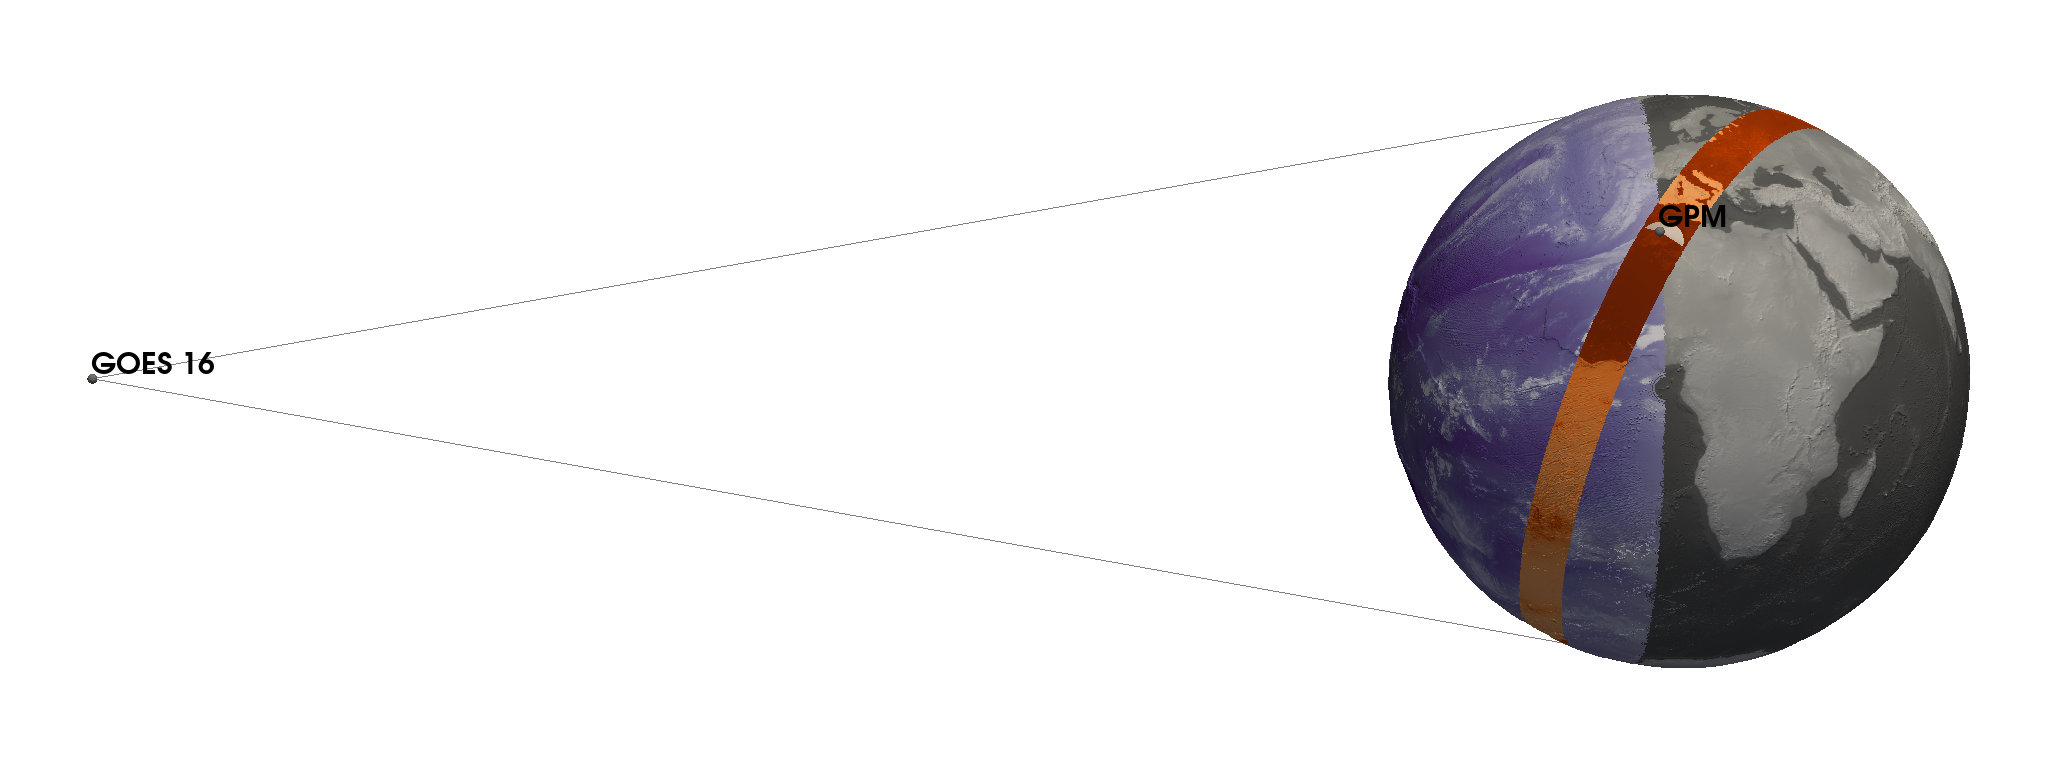
\includegraphics[width=0.8\textwidth]{viewing_geometries}
  \caption{Viewing geometries of geostationary and polar-orbiting satellites
  drawn to scale. The illustration shows geo-located satellite observations from
  the GOES 16 geostationary satellite in purple and from the polar-orbiting GPM
  Core Observatory in orange. The black spheres mark the instantaneous satellite
  positions.}
  \label{fig:remote_sensing:viewing_geometries}
\end{figure}




\subsection{Sensor types}

In addition to \texit{passive} sensors, which sense reflected solar radiation or
thermal radiation emitted from the Earth or its atmosphere, there exist sensors
that themselves emit radiation and measure the amount of it that is scattered
back to the sensor. By measuring the time of travel between emission and
reflection, these \textit{active} sensors measure the distance from the detector
in addition to the intensity of the reflected radiation this allows them to
profile the atmosphere along the line of sight, which leads to much higher
vertical resolutions than what can be achieved with atmospheric sounding.

\subsection{Example: Satllite observations of Hurricane Ida}

Figure~\ref{fig:radiative_transfer:observations} illustrates the different types
of observations used for the remote sensing of hydrometeors using observations
of Hurricane Ida. The first row of panels shows observations derived from the
Advanced Baseline Imager on the GOES 16 geostationary satellite. Panel (a) shows
a natural color composite, which combined observations from 3 channels from the
VIS and NIR to create an image that human color vision. Panel (b) shows
observations from the NIR. Differences in the dielectric constant of water and
ice cause ice clouds to absorb incoming solar radiation much more strongly than
water clouds. The high ice clouds that cover the Hurricane therefore appear much
darker than in the RGB image. Panel (c) shows observation from a window channel
in the FIR. Since it is a window channel, most of the radiation observed in
cloud free areas stems from the Earth's surface and thus appear bright. Where
clouds are present the observed brightness temperatures are closely related to
the atmospheric temperature at the altitude of the cloud and thus colder than
the surface.

Panel (c) and (d) show passive microwave observations at $\SI{18.7}{\giga
  \hertz}$ and $\SI{166}{\giga \hertz}$. At the very low microwave frequencies
only the a thermal emission from precipitation in the hurricane is visible over
the cold ocean surface, while the clouds overland yield no signal. At the higher
microwave frequencies, the surface is not visible due to emission from water
vapor. Scattering by snow particles causes a cold scattering signal from the
thickest clouds around the Hurricane.

Finally, panel (e) shows Ku-band radar reflectivities from the GPM
dual-frequency precipitation radar along a vertical cross section of the
Hurricane. The signal in the radar observations is the amount of energy that is
reflected back to the sensor. Due to the relatively low frequency of the
radar, it is only sensitive to large, precipitation hydrometeors.


\begin{figure}
  \centering
\includegraphics[width=\textwidth]{observations}
\caption{Satellite observations of Hurricane Ida on 2021-08-29 15:09 UTC.
  Panels (a), (b), (c) show observations from the VIS and IR regions obtained
  by the Advanced Baseline Imager on the GOES 16 geostarionary satellite.
  Panels (d) and (e) show passive microwave observations from the GPM microwave
  imager. Panel (f) shows the curtain of radar reflectivity measured by the GPM dual-frequency
  precipitation radar (DPR) along the dashed line shown in panel (a).}
\label{fig:radiative_transfer:observations}
\end{figure}
